%%% Local Variables:
%%% mode: japanese-latex
%%% TeX-engine: uptex
%%% TeX-master: "okuda-master-thesis"
%%% TeX-PDF-mode: t
%%% TeX-PDF-from-DVI: "Dvipdfmx"
%%% End:

\subsection{記号の設定}
本論文の基本的な設定は次のとおりであり,この他に必要な条件は都度明示することとする.

\begin{nttdef}
  \leavevmode\vspace{-1em}
  \begin{itemize}
  \item $\nat,\real, \cpx,\quat$をそれぞれ0を含む自然数全体,実数全体,複素数全体,四元数全体の集合とする.
  \item $G$を非コンパクト実簡約Lie 群,$H$を$G$の非コンパクトかつ連結成分有限個の閉部分群で,$G$のCartan対合$\Theta$に対して$\Theta H = H$なるものとする.
  \item $\ge \defeq \Lie G,\; \ha \defeq \Lie H$とし,$\ge = \ka\oplus \pe$を $\theta \defeq d\Theta$ によるCartan分解とする.
  \item $\ze(\ha)\defeq \{Y\in \ha\mid [Y,\ha] = \{0\} \} $とする.
  \item $e$を$G$の単位元とし,$o_K \defeq eK\in G/K$とする.
  \item $\lyama{-},{-} \ryama$を,$\ge$上の$G$-不変な非退化対称双線型形式で,$\ka$上負定値,$\pe$上正定値で$\ka\perp \pe$なるものとする.
  \item $\per{\ha}\ \defeq \{W\in \ge\mid \lyama W, \ha\ryama = \{0\}\} $とする.
  \item $X\in \pe$に対し,ベクトル空間としての分解$\pe =( \ha\cap \pe)\oplus(\per{\ha}\cap \pe) $に対応した分解を$X = X_1 + X_2 $,$X_1 \in \ha\cap \pe$,$X_2\in \per{\ha}\cap \pe$とする.
  \item $(M,d_M)$を$M$の上の任意の2点に対し一意的な測地線が存在するRiemann多様体と$M$上の計量から定まる距離とする.相異なる点$p,q,r \in M$に対し,
    \begin{itemize}
    \item $\gamma_{p,q}\colon [0, d_{M}(p,q)] \to M$を,$\gamma(0) =  p$,$\gamma(d_{M}(p,q)) = q $なる測地線とする.
    \item $\measuredangle_{p}(q, r)$を$\gamma_{p,q} $と$\gamma_{p,r} $が$p$においてなす角とする.
    \end{itemize}
  \end{itemize}  
\end{nttdef}

以下の\Cref{thm:kob89-lem6.1}を用いて,$X\in \pe$に対し,
\begin{align*}
{(Y(X), Z(X))\defeq \inv{\pi}(e^X\cdot o_K)\in (\ha\cap\pe)\oplus (\per{\ha}\cap \pe)}
\end{align*}
と定義する.
\begin{thm}(\cite[Lemma~6.1]{kob89})\label{thm:kob89-lem6.1}
  \begin{align*}
\pi\colon  (\ha\cap\pe)\oplus (\per{\ha}\cap \pe) \ni (Y, Z)\mapsto e^{Y}e^{Z}\cdot o_K \in G/K
  \end{align*}
  は上への微分同相である.
\end{thm}


ここで,$Y(\real X) $の有界性について,次の\Cref{prob:1121}が小林俊行氏によって提起された.


\begin{prob}(小林俊行氏による)\label{prob:1121}
  ${\pe_{H,\bdd}\defeq \{X\in \pe\mid Y(\real X)\text{ が } \ha\cap \pe \text{ の有界集合である.}  \}}  $と定めるとき,
  \begin{enumerate}
  \item $G$が実半単純Lie群ならば$\pe\setminus\pe_{H,\bdd} $は測度0であるか?
  \item \begin{align}
          \pe_{H,\bdd} = {(\per{\ha}\cap\pe) \cup \{X\in \pe\mid  [X_1, X_2]\neq 0 \text{ かつ }\pe\cap \ze_{\ze(\ha)}(X)  = \{0\} \text{ である.} \}} \label{eq:prob-1121}
        \end{align}
        となっているか?
      \end{enumerate}
\end{prob}

\Cref{prob:1121}についての基本的な事項を挙げる.

\begin{lem}\label{lem:basic-prob}
  \leavevmode\vspace{-1em}
  \begin{enumerate}
  \item ${\pe_{H,\bdd} \subset (\per{\ha}\cap\pe) \cup \{X\in \pe\mid  [X_1, X_2]\neq 0 \text{ かつ }\pe\cap \ze_{\ze(\ha)}(X) = \{0\}  \text{ である.} \}}$が成り立つ.
  \item $X \in \pe $が$X_1 = 0$を満たすならば$X\in \pe_{H,\bdd} $である.
  % \item 1,2より\Cref{prob:1121}と「$X\in \pe$が$[X_1,X_2]\neq 0$ならば$X\in \pe_{H,\bdd} $である」は同値である.
  \item $G$が実階数1ならば,\Cref{prob:1121}と「$\pe_{H,\bdd} =  \{0\}\cup \pe\setminus\ha $」は同値である.
  \end{enumerate}
\end{lem}

\begin{npfwn}[\Cref{lem:basic-prob}]
  \leavevmode\vspace{-1em}
  \begin{enumerate}
  \item $X\nin\per{\ha}\cap \pe $なる$X\in \pe$に対し,$[X_1,X_2] = 0$ならば$e^{tX_1}e^{tX_2}\cdot o_K = e^{t(X_1 + X_2)}\cdot o_K = e^{tX}\cdot o_K$である.したがって\Cref{thm:kob89-lem6.1}より$Y(tX) = tX_1 $,$Z(tX) = tX_2 $であることから$Y(\real X) = \real X_1 $となり,$X_1\neq 0$より$Y(\real X)$は有界集合とならない.


  \item $X_1 = 0$であることと$ X\in \per{\ha}\cap\pe $であることが同値であることから従う.
  \item $G$が実階数1として次を示せばよい.
    \begin{align}
      \{0\}\cup \pe\setminus \ha = (\per{\ha}\cap\pe) \cup \{X\in \pe\mid  [X_1, X_2]\neq 0 \text{ かつ } \pe\cap \ze_{\ze(\ha)}(X) = \{0\}  \text{ である.} \}\label{eq:basic-prob}
    \end{align}
    $G$の実階数が1かつ$H$が非コンパクトであるから$\ha\cap\pe$は極大分裂可換部分代数であり,右辺の2つ目の集合は$\ze(\ha)\cap\pe \subset \real X_{1}\neq \{0\} $より$\{X\in \pe\mid  [X_1, X_2]\neq 0 \}$となる.よって\Cref{eq:basic-prob}の右辺は$\{X\in \pe\mid X_1 = 0\text{ または }  [X_1, X_2]\neq 0 \text{ である.} \}$と同値である.この集合はさらに$X\in \{0\}\cup\pe\setminus\{0\} $と同値であるから\Cref{eq:basic-prob}が示された.
  \end{enumerate}  
\end{npfwn}

$Y(\real X) $の有界性は$\Ad(k) $-不変である.具体的には\Cref{lem:1101}が成り立つ.
\begin{lem}\label{lem:1101}
  $k\in K$,$X\in \pe$に対し,$X'\defeq \Ad(k)X $,$\ha'\defeq \Ad(k)\ha $とする.$Y'(X'), Z'(X') $を,微分同相$\pi'\colon (\ha'\cap \pe)\oplus (\per{\ha'}\cap \pe)\ni (Y',Z')\mapsto e^{Y'}e^{Z'}\cdot o_K  $を用いて,$X'\in \pe$に対し,$(Y'(X'), Z'(X')) = \inv{\pi'}(e^{X'}\cdot o_K) $と定める.

  このとき$Y(\real X)$が有界であることと$ Y'(\real X') $が有界であることは同値である.
\end{lem}

\begin{npfwn}[\Cref{lem:1101}]
  主張は$(X,\ha) $と$(X',\ha')$に対して対称的であるから,$Y(\real X) $が有界ならば$Y'(\real X') $が有界であることのみを示せば十分である.

  任意に$r\in \real$を取る.$e^{rX'}\cdot o_K = e^{Y'(r X')}e^{Z'(r X')}\cdot o_K  $であり,両辺に左から$\inv{k} $を掛けると,$e^{r X} = e^{\Ad(\inv{k})( Y'(r X'))}e^{\Ad(\inv{k})( Z'(r X'))}\cdot o_K  $を得る.ここで$Y'(rX')\in \ha'\cap \pe $,$Z'(r X')\in \per{\ha'}\cap \pe $であるから$\Ad(\inv{k})(Y'(r X'))\in \ha\cap \pe $,$\Ad(\inv{k})(Z'(r X')) \in \per{\ha}\cap \pe $である.

  \Cref{thm:kob89-lem6.1}により$\pi$は微分同相であるから,任意の$r\in \real$に対して$\Ad(\inv{k})(Y'(r X')) = Y(rX)  $である.$Y'(\real X) = \Ad(k)(Y(\real X))  $であり,$\Ad(k) $は有限次元空間の間の線型写像であるから有界性を保つ.

  以上から\Cref{lem:1101}が示された.  
\end{npfwn}


$Y(\real X) $の有界性を判定しようとする\Cref{prob:1121}と比較して$Z(\real X) $の有界性については次の定理が知られており,有界性の判定はLie環の言葉のみで行える.

\begin{thm}(\cite[Lemmma~5.4]{kob97})\label{thm:kob97}
  $X\in \pe$に対し,$\norm{Z(X)}\geq \norm{X} \sin\phi(X, \ha\cap\pe)$である.ここに$\phi(X,\ha\cap \pe) $は$X$と$\ha\cap \pe$の元がなす角度の最小値${0\leq \phi(X,\ha\cap \pe) \leq \frac{\pi}{2}} $であり,$X\in \pe\setminus \ha \iff \phi(X,\ha\cap \pe)\neq 0 $である.
\end{thm}

\Cref{thm:kob97}より,$X\in \ha $と$Z(\real X) $が有界であることが同値である.


\subsection{\Cref{prob:1121}の観察: $G = \SU(1,1) $,$H = \SO(1,1) $の場合}

$G = \SU(1,1) $,$H = \SO(1,1) \defeq\lbig\{
\begin{pmatrix}
  \cosh t & \sinh t\\ \sinh t & \cosh t
\end{pmatrix}
\relmiddle| t\in \real \rbig\} $の場合に\Cref{prob:1121}が正しいことは直接計算により確かめられる.

\begin{prop}\label{prop:prob-eg}
  $G = \SU(1,1) $,$H = \SO(1,1) $のとき\Cref{prob:1121}は正しい.
\end{prop}

% \bluetext{$\sulie(1,1) $のKilling形式と$r = \tanh t$の関係を明記せよ.}

\begin{lem}\label{lem:riem-metric-su11}
  $\ge\defeq \sulie(1,1)$のKilling形式から定まる{\Poincare}円板${G/K =\{x+\sqrt{-1}y\mid  x^2 + y^2 < 1 \} }$の計量は$ \dfrac{8(dx^2 + dy^2)}{(1 - x^2 - y^2)^2} $である.
\end{lem}

\begin{npfwn}[\Cref{lem:riem-metric-su11}]
  
  $\ge$の元を$G/K$上の左不変ベクトル場と同一視すると
  \begin{align*}
    X' &\defeq 
         \begin{pmatrix}
           0 & 1 \\ 1 & 0
         \end{pmatrix} = \dfrac{\del}{\del x},\\
    Y' &\defeq 
         \begin{pmatrix}
           0 & \sqrt{-1} \\ -\sqrt{-1} & 0
         \end{pmatrix} = \dfrac{\del}{\del y}
  \end{align*}
  である.$\ge$のKilling形式$B$から定まる$\pe$上のノルム$\norm{-} $に対して$\norm{X'}^2 = \norm{Y'}^2 = 8 $,$B(X', Y' ) = 0$であって,$0\in G/K =\{x+\sqrt{-1}y\mid x^2 + y^2 < 1 \}  $で主張が成り立つ.

  したがって$k_{\theta} \defeq \diag(e^{\sqrt{-1}\theta},e^{-\sqrt{-1}\theta}) $,$a_r\defeq
  \begin{pmatrix}
    \cosh r & \sinh r \\  \sinh r & \cosh r
  \end{pmatrix}
  $とすると,
  \begin{align*}
    &g(d\tau(k_{\theta/2}a_r)(d\tau(k_{-\theta/2})X'), d\tau(k_{\theta/2}a_r)(d\tau(k_{-\theta/2})X')) \\
    =&\ g (d\tau(k_{\theta/2}a_r)(d\tau(k_{-\theta/2})Y'), d\tau(k_{\theta/2}a_r)(d\tau(k_{-\theta/2})Y')) \\
    =&\ 8, \\
    &g(d\tau(k_{\theta/2}a_r)(d\tau(k_{-\theta/2})X'), d\tau(k_{\theta/2}a_r)(d\tau(k_{-\theta/2})Y'))  = 0
  \end{align*}
  なるような計量$g $がKilling形式から誘導される計量であるが,それが主張の形であることを示せば良い (これらのベクトルが何を表しているかは\Cref{fig:riem-metric-su11}参照).

  \begin{figure}[H]
    \centering
    % \raggedleft
    % \raggedrightp
    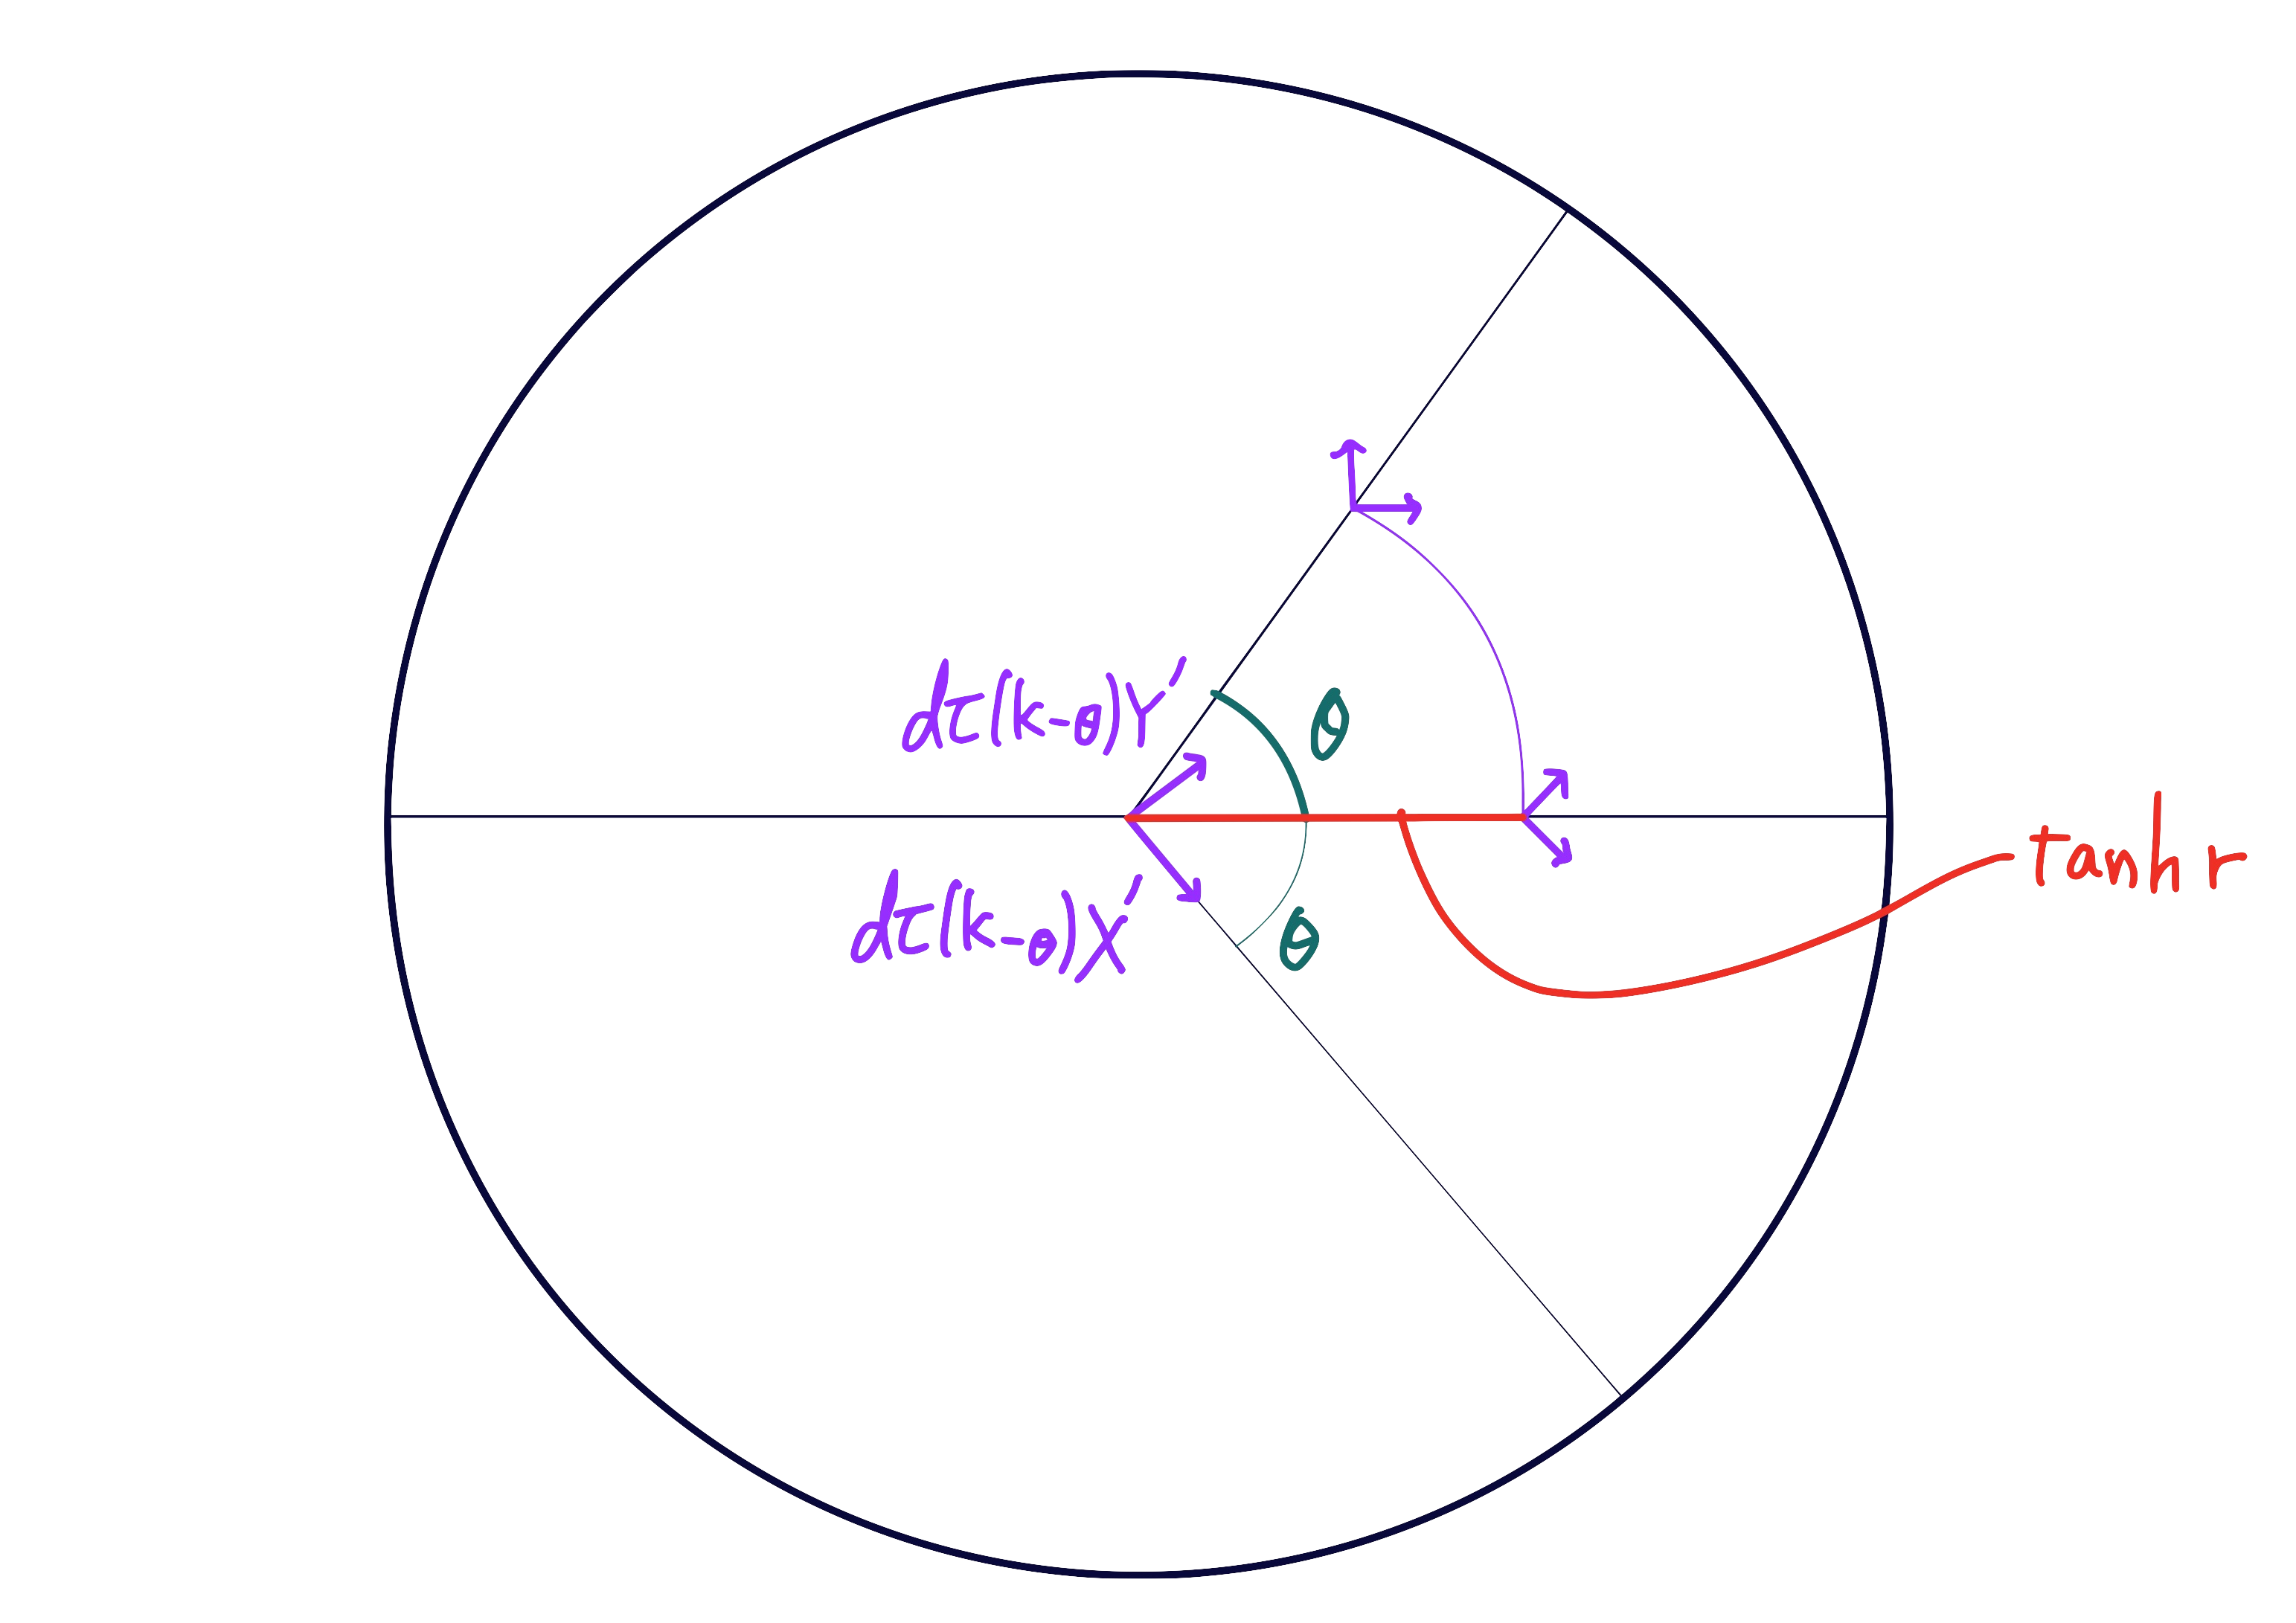
\includegraphics[scale=0.08]{../graph/riem-su11.png}
    % 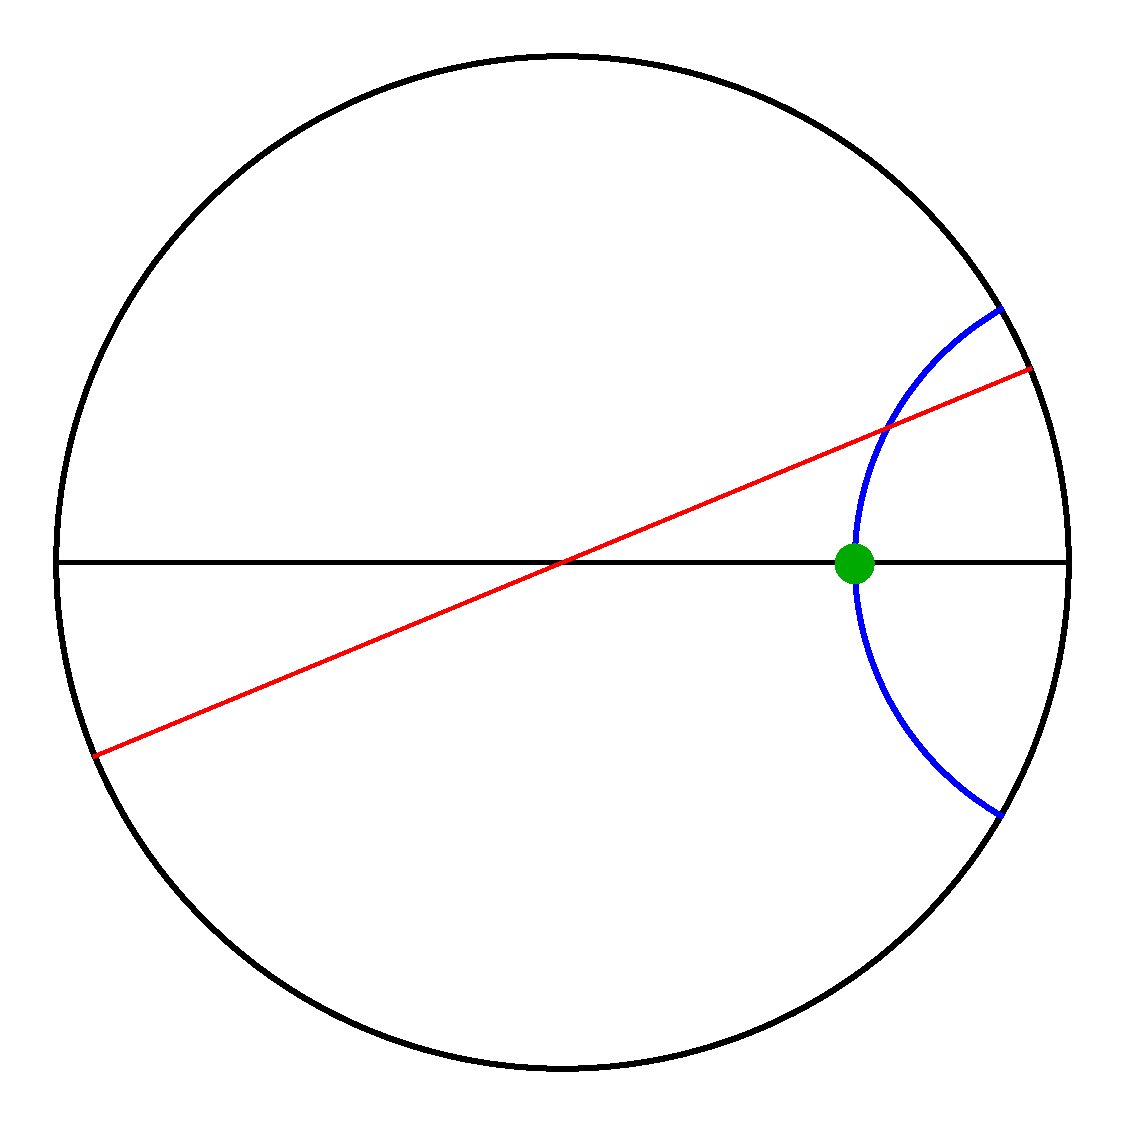
\includegraphics[scale=0.3]{../graph/y-and-z.pdf}
    \caption{}
    \label{fig:riem-metric-su11}
  \end{figure}


  $t = 0$での接ベクトルが$d\tau(k_{\theta/2}a_r)d\tau(k_{-\theta/2})X'$を与える曲線は
  \begin{align*}
    \gamma_x(t) \defeq  e^{\sqrt{-1} \theta}\dfrac{\cosh r\cdot e^{-\sqrt{-1}\theta} \tanh t + \sinh r }{\sinh r\cdot e^{-\sqrt{-1}\theta} \tanh t + \cosh r}
  \end{align*}
  であるから,
  \begin{align*}
    \lbig.\dfrac{d}{dt}\rbig|_{t=0}\gamma_x(t) = d\tau(k_{\theta/2}a_r)d\tau(k_{-\theta/2})X' = (1 - \tanh^2 r)\dfrac{\del}{\del x} = (1-x^2-y^2)\dfrac{\del}{\del x}
  \end{align*}
  である.

  同様に$t = 0$での接ベクトルが$d\tau(k_{\theta/2}a_r)d\tau(k_{-\theta/2})Y'$を与える曲線は
  \begin{align*}
    \gamma_y(t) \defeq  e^{\sqrt{-1} \theta}\dfrac{\cosh r\cdot e^{-\sqrt{-1}\theta}\sqrt{-1} \tanh t + \sinh r }{\sinh r\cdot e^{-\sqrt{-1}\theta}\sqrt{-1} \tanh t + \cosh r}
  \end{align*}
  であるから,
  \begin{align*}
    \lbig.\dfrac{d}{dt}\rbig|_{t=0}\gamma_y(t) = d\tau(k_{\theta/2}a_r)d\tau(k_{-\theta/2})Y' = (1 - \tanh^2 r)\dfrac{\del}{\del y} = (1-x^2-y^2)\dfrac{\del}{\del y}
  \end{align*}
  である.

  以上より$g  =  \dfrac{8(dx^2 + dy^2)}{(1 - x^2 - y^2)^2} $が示された.
\end{npfwn}


\begin{npfwn}[\Cref{prop:prob-eg}]


  $k_{\theta} \defeq \diag(e^{\sqrt{-1}\theta},e^{-\sqrt{-1}\theta}) $,$X_{\theta} \defeq k_{\theta/2}
  \begin{pmatrix}
    0 & 1 \\ 1 & 0
  \end{pmatrix}
  k_{-\theta/2}$とすると,$\pe\setminus\{0\} =  \{tX_{\theta}\mid t\in \real_{>0},\ 0\leq \theta\leq \pi\}$である.この$X_{\theta} $と$t\in \real$に対して$Y(tX_{\theta} ) = s
  \begin{pmatrix}
    0 & 1 \\ 1 & 0
  \end{pmatrix}
  $なる$s\in \real $を求める.


  
  \begin{figure}[H]
    \centering
    % \raggedleft
    % \raggedrightp
    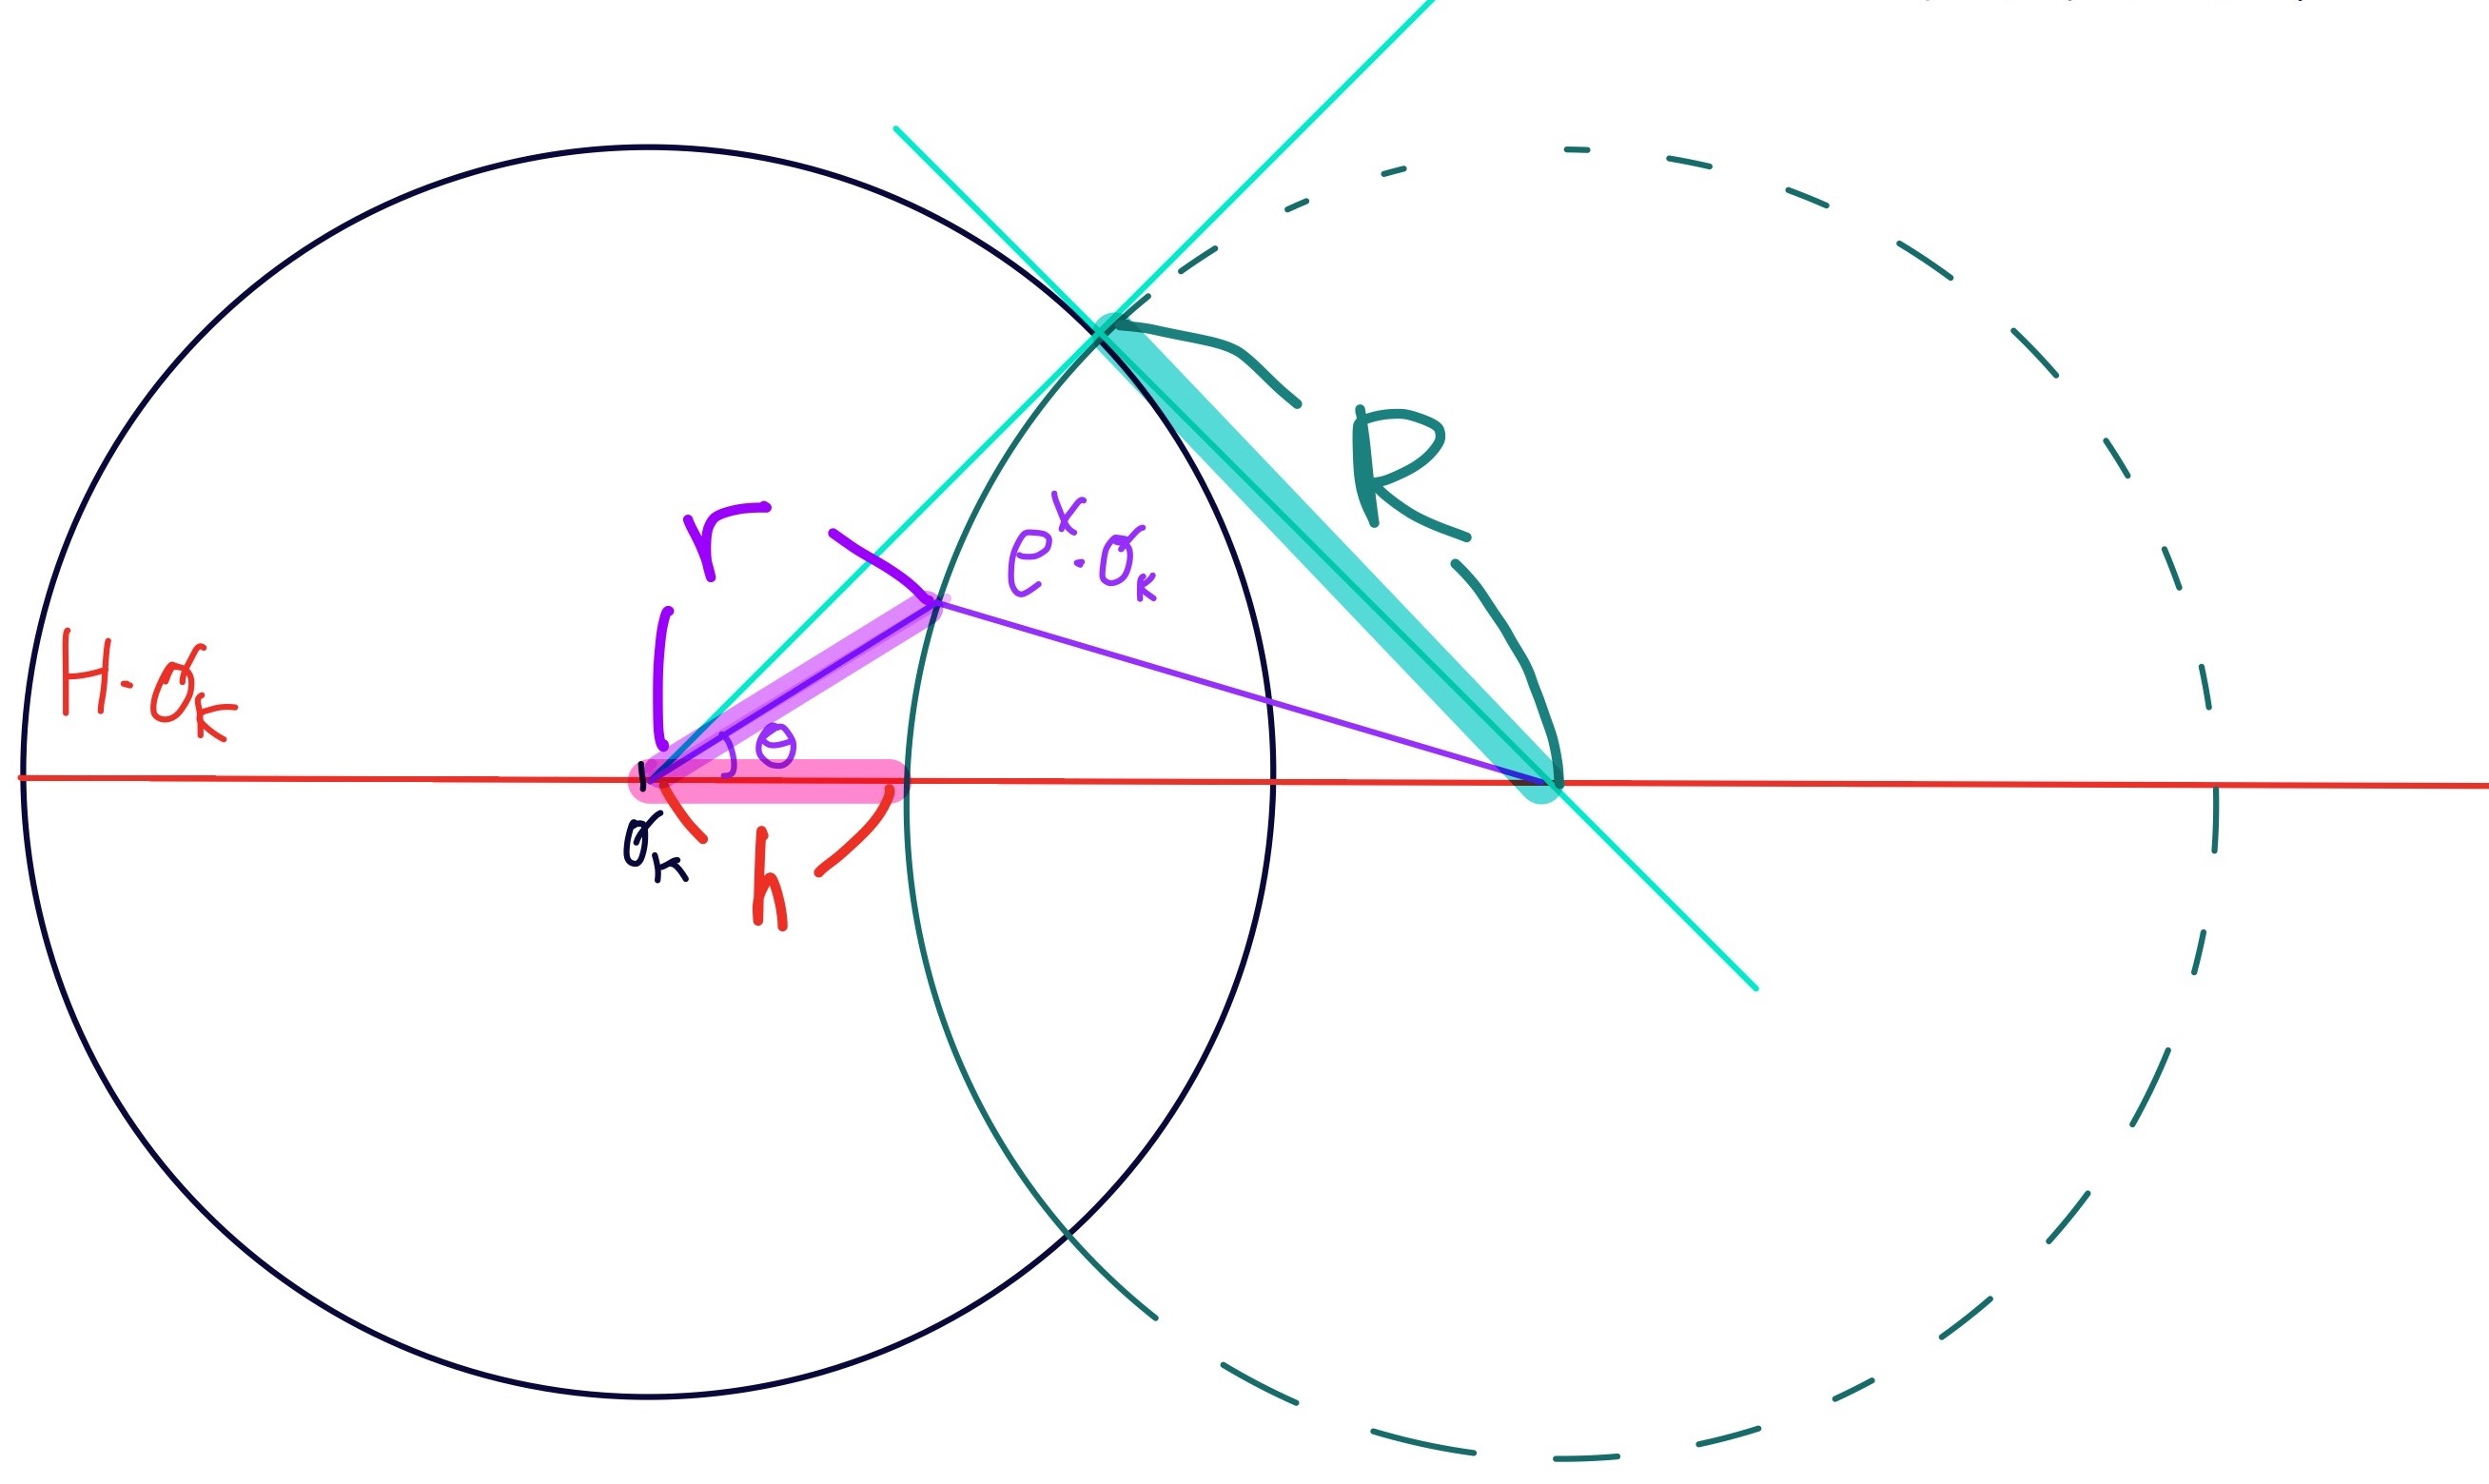
\includegraphics[scale=0.08]{../graph/prob-eg-1.jpg}
    % 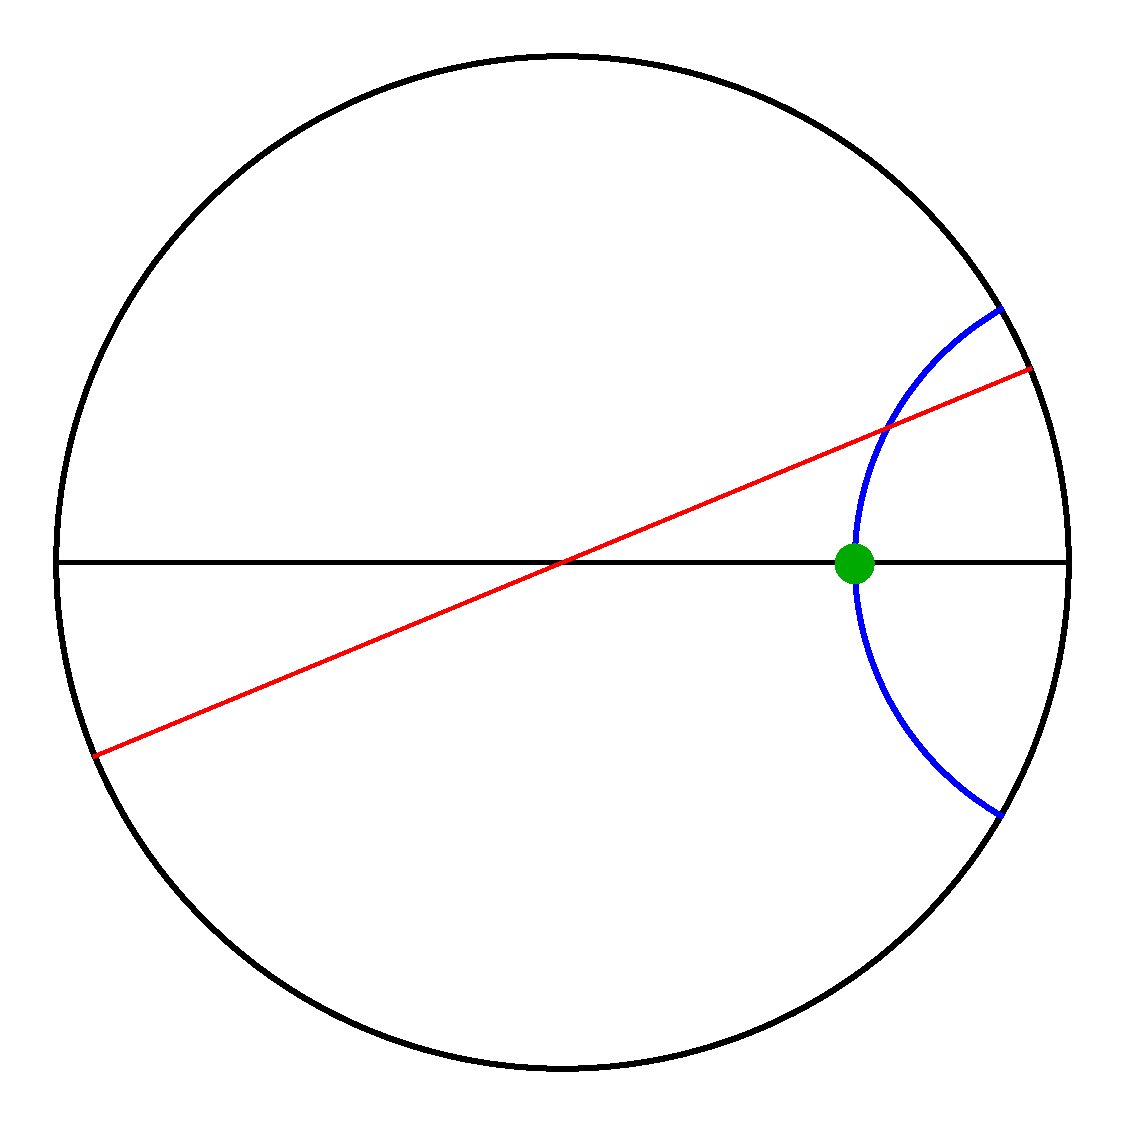
\includegraphics[scale=0.3]{../graph/y-and-z.pdf}
    \caption{}
    \label{fig:prob-eg-1}
  \end{figure}

  右の円の Euclid 距離での半径を$R$とし,$e^{tX_{\theta}}\cdot o_K $から$H\cdot o_K$への垂線の足の$o_K$からの Euclid 距離を$h$とするとき,外側の青色の直角三角形に対して三平方の定理を用いて$(h+R)^2 = R^2 +  1 $より$R = \dfrac{1-h^2}{2h}$,$R+h = \dfrac{1+h^2}{2h}  $を得る.

  さらに下の紫色の三角形に対して余弦定理を用いて${R^2 = (R+h)^2 + r^2 - 2(R+h) \cos\theta }$を得,
  \begin{align}
    {\dfrac{2r\cos\theta}{r^2 + 1} = \dfrac{2h}{h^2 + 1} }\label{eq:1018-main}
  \end{align}
  を得る.

  $r = \tanh t$,$h = \tanh s$であるから\Cref{eq:1018-main} は$\cos\theta \tanh 2t = \tanh 2t $と書き直せる.したがって$X_{\theta}$に対して$Y(\real X) $が有界$\iff \abs{\cos\theta}\neq 1 \iff  X\nin \ha  $である.
\end{npfwn}

\begin{rem}\label{rem:su11-by-angle}

  \Cref{prop:prob-eg}は角度を用いた議論によっても示すことができる.具体的には,計算により次の\Cref{lem:0106}が示せる.
  \begin{lem}\label{lem:0106}
    $e^{sY}e^{rZ}\cdot o_K =
    \begin{pmatrix}
      \cosh s & \sinh s\\ \sinh s & \cosh s
    \end{pmatrix}
    \sqrt{-1}\tanh r \in \SU(1,1)/\U(1) $,$s > 0$,$r\in \real$に対し,$\phi_{s,r}\defeq \measuredangle_{o_K}(e^{sY}e^{rZ}\cdot o_K, e^{sY}\cdot o_K) $は,$\tan \phi_{s,r} = \dfrac{\tanh 2r}{\sinh 2s} $を満たす.ただし$Y \defeq
  \begin{pmatrix}
    0 & 1\\ 1 & 0
  \end{pmatrix}
  $,$Z \defeq \begin{pmatrix}
    0 & \sqrt{-1} \\ -\sqrt{-1} & 0
  \end{pmatrix}$とする.
  \end{lem}  

  \Cref{lem:0106}により\Cref{prop:prob-eg}は次のように証明できる.
  任意の$0\neq s\in \real, r\in \real $に対し,
  \begin{align}
    \lim_{r\to -\infty}\tan \phi_{\abs{s},r} = \dfrac{-1}{\sinh 2\abs{s}}  \leq \tan \phi_{s,r} \leq  \lim_{r\to \infty}\tan \phi_{\abs{s},r} = \dfrac{1}{\sinh 2\abs{s}}\label{eq:0106}
  \end{align}
  であるから,$X\nin \real Y $の元に対して$Y(\real X) $が非有界であるとすると,$ 0 <  \epsilon < \phi(X,\ha)$なる$\epsilon$に対し,ある$t\in \real $が存在して,$Y(tX) = s_tY $,$\sinh 2\abs{s_t} > \dfrac{1}{\tan \epsilon} $である.$Z(tX) = r_tZ $とすると\Cref{eq:0106}より$\abs{\tan \phi_{s_t,r_t}} < \tan \epsilon $,したがって
  \begin{align*}
    -\epsilon < \measuredangle_{o_K}(e^{s_tY}e^{r_t Z}\cdot o_K, e^{s_tY}\cdot o_K) < \epsilon < \phi(X,\ha)
  \end{align*}
  となる.しかし定義より$\measuredangle_{o_K}(e^{s_tY}e^{r_t Z}\cdot o_K, e^{s_tY}\cdot o_K) = \measuredangle_{o_K}(e^{tX}\cdot o_K, e^{Y(tX) }\cdot o_K) $であり,$\measuredangle_{o_K}(e^{tX}\cdot o_K, e^{Y(tX) }\cdot o_K) = \phi(X,\ha)$であるから矛盾する.

  
\end{rem}

\begin{cor}\label{cor:prob-eg}
  $G = \SO(1,n) $,$H = \SO(1,k) $,$1\leq k\leq n-1$に対して\Cref{prob:1121}は正しい.
\end{cor}


\begin{npfwn}[{\Cref{cor:prob-eg}}]\bluetext{make it precise}
  $\SO(1,n)/\SO(n)$の開球としての実現を考える.「$e^X\cdot o_K $と$o_K$を結ぶ直線」と$H\cdot o_K$で張られる超平面で$\SO(1,n)/\SO(n)$を切った際の断面を考える.
  \begin{figure}[H]
    \centering
    % \raggedleft
    % \raggedrightp
    % \includegraphics[scale=0.08]{../graph/fig1.jpg}
    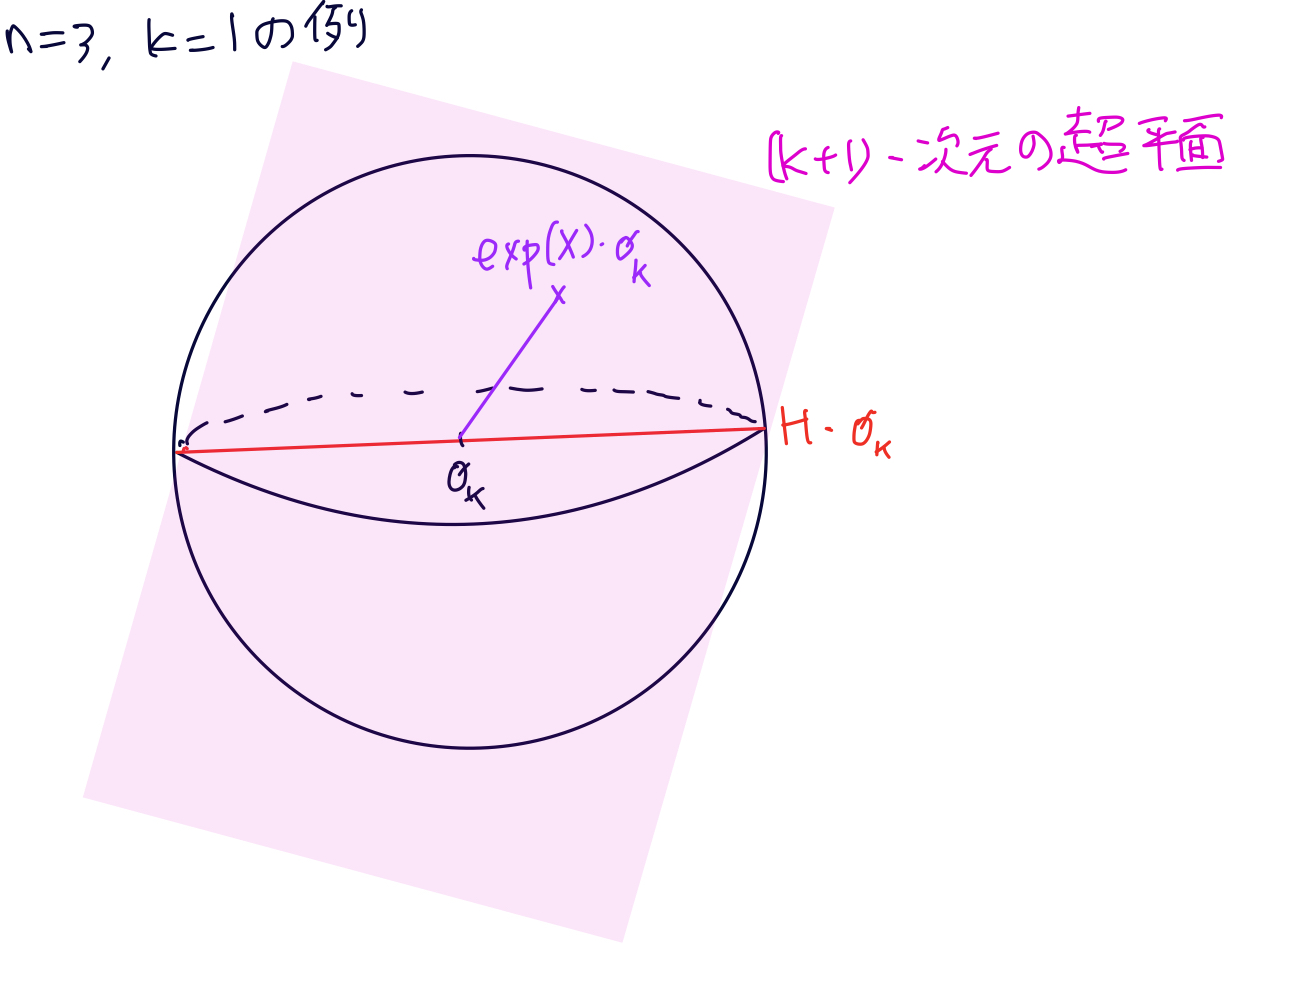
\includegraphics[scale=0.2]{../graph/son1-3.jpeg}
    \caption{}
    \label{fig:son1}
  \end{figure}
  
  この断面に現れるのは\Cref{fig:prob-eg-1}と同じであるから,同様の計算により\Cref{cor:prob-eg}を得る.
\end{npfwn}


\subsection{\Cref{prob:1121} の観察: 類似の問いとその反例}

\Cref{prob:1121}は,$G$の実階数が1の場合は
\begin{prob}\label{prob:1121-2}

  $\pe_{H,\bdd} = \{X\in \pe\mid [X,(\ha\cap\pe)]\neq \{0\} \text{ あるいは } X\perp (\ha\cap\pe)\text{ である.}  \}  $となるか?
  
\end{prob}
と同値であった.しかし\Cref{prob:1121-2}には$G$の実階数が2の場合の反例が存在する.
\begin{prop}\label{prop:0114}
  $G = \SL(3,\real) $,$H = \{\diag(e^a,e^b,e^c)\mid a,b,c\in \real,\ a+ b + c = 0 \} $,$X\defeq
  \begin{pmatrix}
    1 & 0 & 0 \\
    0 & 0 & \sqrt{2} \\
    0 & \sqrt{2} & -1
  \end{pmatrix}
  $に対し$Y(\real X) $は非有界である.
\end{prop}


$\ha = \{\diag(a,b,c)\mid a,b,c\in \real,\ a +b + c = 0 \}  $であるから$X_1 = \diag(1,0,-1)$,$X_2 = \begin{pmatrix}
  0 & 0 & 0 \\
  0 & 0 & \sqrt{2} \\
  0 & \sqrt{2} & 0
\end{pmatrix}$であり,$[X_1, X_2] = \begin{pmatrix}
  0 & 0 & 0 \\
  0 & 0 & \sqrt{2} \\
  0 & -\sqrt{2} & 0
\end{pmatrix} \neq 0$より$X$は\Cref{eq:prob-1121}の右辺の集合の元ではあるが$X\nin \pe_{H,\bdd} $であるから,\Cref{prop:0114}は\Cref{prob:1121}の反例となっている.

1つ補題を用意してから\Cref{prop:0114}を証明する.
\begin{lem}\label{lem:0114}
  任意の$t\in \real$に対し
  \begin{align*}
    \exp\lbig(2t\begin{pmatrix}
      0 & \sqrt{2} \\
      \sqrt{2} & -1 
    \end{pmatrix}\rbig) &=
                 \begin{pmatrix}
                   \dfrac{2e^{2t} + e^{-4t}}{3} &  \dfrac{\sqrt{2} (e^{2t} - e^{-4t})}{3}\\
                   \\
                   \dfrac{\sqrt{2} (e^{2t} - e^{-4t})}{3} & \dfrac{e^{2t} + 2e^{-4t}}{3}
                 \end{pmatrix}
  \end{align*}
  である.
\end{lem}

\begin{npfwn}[\Cref{lem:0114}]

  $ \theta $を$\cos 2\theta = \dfrac{1}{3} $,$\sin 2\theta = \dfrac{-2\sqrt{2}}{3} $を満たす実数として任意に1つ固定する.このとき
  \begin{align*}
    \cos^2 \theta &= \dfrac{1 +\cos 2\theta}{2} = \dfrac{2}{3},\\
    \sin^2 \theta &= \dfrac{1-\cos 2\theta}{2} = \dfrac{1}{3}
  \end{align*}
  である.$k \defeq
  \begin{pmatrix}
    \cos \theta & -\sin \theta \\ \sin \theta & \cos \theta
  \end{pmatrix}
  $とすると,
  \begin{align*}
    k
    \begin{pmatrix}
      0 & \sqrt{2} \\
      \sqrt{2} & -1 
    \end{pmatrix}\inv{k} &=
                           \begin{pmatrix}
                             -2\sqrt{2}\sin\theta \cos\theta  - \sin^2\theta & \sqrt{2}(\cos^2 \theta - \sin^2\theta) + \cos\theta \sin\theta \\
                             \sqrt{2}(\cos^2 \theta - \sin^2\theta) + \cos\theta \sin\theta  & 2\sqrt{2}\sin\theta \cos\theta  - \cos^2\theta
                           \end{pmatrix}\\
        &=
          \begin{pmatrix}
            -\sqrt{2}\sin 2\theta  - \sin^2\theta & \sqrt{2}\cos 2\theta + \dfrac{\sin 2\theta}{2} \\
            \sqrt{2}\cos 2\theta + \dfrac{\sin 2\theta}{2}  &\sqrt{2}\sin 2 \theta - \cos^2\theta
          \end{pmatrix}\\
        &=
          \begin{pmatrix}
            1  &  0\\ 0 & -2
          \end{pmatrix}
  \end{align*}
  である.

  したがって
  \begin{align*}
    k\exp\lbig(2t\begin{pmatrix}
      0 & \sqrt{2} \\
      \sqrt{2} & -1 
    \end{pmatrix}\rbig)\inv{k} &= \exp
                                 \begin{pmatrix}
                                   2t & 0 \\ 0 & -4t
                                 \end{pmatrix}
  \end{align*}
  であるから,
  \begin{align*}
    \exp\lbig(2t\begin{pmatrix}
      0 & \sqrt{2} \\
      \sqrt{2} & -1 
    \end{pmatrix}\rbig) &= \inv{k} \exp\lbig(
                                 \begin{pmatrix}
                                   2t & 0 \\ 0 & -4t
                                 \end{pmatrix}\rbig)k\\
        &=
          \begin{pmatrix}
            \cos \theta  & \sin \theta \\ -\sin \theta & \cos \theta
          \end{pmatrix}
                                                         \begin{pmatrix}
                                                           e^{2t} & 0 \\ 0 & e^{-4t}
                                                         \end{pmatrix}
                                                                             \begin{pmatrix}
                                                                               \cos \theta  & -\sin \theta \\ \sin \theta & \cos \theta
                                                                             \end{pmatrix}\\
        &=
          \begin{pmatrix}
            e^{2t}\cos^2\theta + e^{-4t}\sin^2 \theta  & (e^{-4t} - e^{2t})\sin\theta \cos\theta \\ (e^{-4t} - e^{2t})\sin\theta \cos\theta  & e^{2t}\sin^2\theta +e^{-4t}\cos^2\theta
          \end{pmatrix}\\
        &= \begin{pmatrix}
          \dfrac{2e^{2t} + e^{-4t}}{3} &  \dfrac{\sqrt{2} (e^{2t} - e^{-4t})}{3}\\
          \\
          \dfrac{\sqrt{2} (e^{2t} - e^{-4t})}{3} & \dfrac{e^{2t} + 2e^{-4t}}{3}
                 \end{pmatrix}
  \end{align*}
\end{npfwn}

\begin{npfwn}[\Cref{prop:0114}]
  行列式1の$3\times 3$正定値実対称行列全体の集合$\Symm^{+}(3)$と$G/K$は$gK \mapsto g
  \begin{pmatrix}
    1 & 0\\ 0 & 1
  \end{pmatrix}
  \trans{g} $により微分同相である.
  
  \Cref{lem:0114}より
  \begin{align}
    e^{tX}\cdot o_K &= e^{tX}\; \trans{(e^{tX})} = e^{2tX}\notag\\
                    &= \begin{pmatrix}
                      e^{2t} & 0 & 0 \\
                      0 & \dfrac{2e^{2t} + e^{-4t}}{3} &  \dfrac{\sqrt{2} (e^{2t} - e^{-4t})}{3}\\
                      % \\
                      0 & \dfrac{\sqrt{2} (e^{2t} - e^{-4t})}{3} & \dfrac{e^{2t} + 2e^{-4t}}{3}
                    \end{pmatrix}\label{eq:0114-1}
  \end{align}
  である.

  $Y \defeq \diag(a,b,c)  $,$a + b + c = 0$,$Z \defeq
  \begin{pmatrix}
    0 & 0 & 0\\
    0 & 0 & 1\\
    0 & 1 & 0
  \end{pmatrix}
  $とすると,$r\in \real$に対し,
  \begin{align}
    e^{Y}e^{rZ}\cdot o_K &= e^{Y}e^{2rZ}e^{Y}\notag\\
                         &=
                           \begin{pmatrix}
                             e^{a} & 0 & 0 \\
                             0 & e^{b} & 0\\
                             0 & 0 & e^{c}
                           \end{pmatrix}
                                     \begin{pmatrix}
                                       1 & 0 & 0\\
                                       0 & \cosh 2r & \sinh 2r \\
                                       0 & \sinh 2r & \cosh 2r
                                     \end{pmatrix}
                                                      \begin{pmatrix}
                                                        e^{a} & 0 & 0 \\
                                                        0 & e^{b} & 0\\
                                                        0 & 0 & e^{c}
                                                      \end{pmatrix}\notag\\
                         &=
                           \begin{pmatrix}
                             e^{2a} & 0 & 0\\
                             0 & e^{2b}\cosh 2r & e^{b+c}\sinh 2r \\
                             0 & e^{b+c}\sinh 2r & e^{2c}\cosh 2r
                           \end{pmatrix}\notag\\
                         &= \begin{pmatrix}
                             e^{2a} & 0 & 0\\
                             0 & e^{2b}\cosh 2r & e^{-a}\sinh 2r \\
                             0 & e^{-a}\sinh 2r & e^{-2a-2b}\cosh 2r
                           \end{pmatrix}\label{eq:0114-2}
  \end{align}
  である.ただし最後の変形には$a + b + c = 0$を用いた.

  \Cref{eq:0114-1}と\Cref{eq:0114-2}を見比べると,
  \begin{align*}
    a &= t,\\
    \sinh 2r &= \dfrac{2\sqrt{2}}{3}\sinh 3t, \\
    e^{2b} &= \dfrac{2e^{2t} + e^{-4t}}{\sqrt{9 + 8\sinh^2 3t}}
  \end{align*}
  とすると$e^{Y}e^{rZ}\cdot o_K = e^{tX}\cdot o_K $を得る.つまり任意の$t\in \real$に対し
  \begin{itemize}
  \item $Y(tX) = \diag(a(t) ,b(t) ,-a(t) -b(t) ) $

    ただし$a(t) = t$,$b(t) =\dfrac{1}{2} \log \lbig(\dfrac{2e^{2t} + e^{-4t}}{\sqrt{9 + 8\sinh^2 3t}}\rbig) $,
  \item $Z(tX) = r(t)Z  $ただし$r(t) = \dfrac{1}{2} \inv{\sinh}\lbig( \dfrac{2\sqrt{2}}{3}\sinh 3t\rbig) $
  \end{itemize}
  であるから,$Y(\real X) $は非有界である.  
\end{npfwn}



$G$が実階数1の場合に限っても\Cref{prob:1121-2}と類似の問題はいくつか考えられる.例えば$\ha\cap\pe$を$\ha$に置き換えた次の問題が立てられる.
\begin{prob}\label{prob:1101}
  $\pe_{H,\bdd} = \{X\in \pe\mid  [X,\ha]\neq \{0\} \text{ あるいは } X\perp \ha \text{ である.}\}  $となるか?
\end{prob}

しかし\Cref{prob:1101}にも反例が存在する.
\begin{lem}\label{lem:1118-main}
  $G = \SL(3,\real) $,$Y_1\defeq \diag(1,1,-2)$,$Y_2 \defeq \begin{pmatrix}
    0 & 1 & 0\\
    -1 & 0 & 0 \\
    0 & 0 & 0
  \end{pmatrix}$,\\
  $\ha = \real Y_1 \oplus \real Y_2 $,$X = \diag(1,0,-1) $に対し,$[X,\ha] \neq \{0\} $であるが$Y(\real X) = \real Y_1 $であり,非有界である.
\end{lem}

\begin{ncalcof}[\Cref{lem:1118-main}]

  $\ha$は可換Lie環であり,$\ge = \slie(3,\real) $のCartan対合$\theta W \defeq -\trans{W} $に対し$\ha = \theta \ha$である.

  $[X,\ha]\neq 0 $は,$[X, Y_2] \neq 0$より従う.

  ここで$Z_1\defeq \diag(1,-1,0)\in \per{\ha}\cap \pe $であり,任意の$t\in \real$に対し,$e^{2tX} = e^{tY_1}e^{tZ_1} $であるから,$Y(\real X) = \real Y_1 $となり,\Cref{lem:1118-main} が示された.
\end{ncalcof}

\Cref{lem:1118-main}において$X$と$\ha$は,$[X,\ha] \neq \{0\} $だが$[X,(\ha\cap \pe)] = \{0\}$かつ$X\not\perp (\ha\cap \pe) $となるように取った.したがって\Cref{prob:1101}の右辺を次の\Cref{prob:1101-2}のように少し弱めても\Cref{lem:1118-main}はその反例になっている.
\begin{prob}\label{prob:1101-2}
  $\pe_{H,\bdd} = \{X\in \pe\mid  [X,\ha]\neq \{0\} \text{ あるいは } X\perp (\ha\cap\pe) \text{ である.} \}  $となるか?
\end{prob}
